\chapter{Introducción al cálculo simbólico\\Introduction to symbolic computing}\index{Cálculo Simbolico}
\chaptermark{Intro cálculo simbólico  \textreferencemark\ Intro symbolic computing}
\epigraph{And earthly power doth then show likest God's
	When mercy seasons justice.}{The merchan of Venice, Willian Shakespeare}

\begin{paracol}{2}
En este último capítulo vamos a introducir un método de cálculo que difiere notablemente de lo visto  en los capítulos anteriores: se trata del cálculo simbólico. Hasta ahora, hemos empleado siempre el ordenador para hacer cálculo numérico. Las variables se definían asignándoles un valor numérico y después eran empleadas en operaciones algebraicas o se les aplicaban funciones matemáticas para obtener a partir de ellas resultados numéricos.

Sin embargo, en matemáticas y en física, es práctica habitual realizar operaciones con variables y funciones sin asignarles un resultado numérico. Un ejemplo típico es el de la derivación de una función,
\end{paracol}
\begin{equation*}
f(x) = \sqrt{1-\ln x} \rightarrow f'(x) =-\frac{1}{2x\sqrt{1 - \ln x}} 
\end{equation*}  
\begin{paracol}{2}
A partir de una expresión \emph{simbólica} de la función obtenemos su derivada expresada también de modo \emph{simbólico} como otra función. También con un computador es posible hacer este tipo de operaciones, a las que se da el nombre de cálculo simbólico para distinguirlas del cálculo numérico.  
\end{paracol}

\begin{paracol}{2}
\section{Cálculo simbólico con Sympy}
Sympy  es un módulo de Python creado para realizar cálculo simbólico. Como en el caso de otros módulos que hemos introducido en capítulos anteriores, nos vamos a limitar a dar una introducción al cálculo simbólico empleando Sympy, para conocer de verdad sus posibilidades se aconseja acudir a la documentación del módulo, disponible en interner
\section{Variables y expresiones simbólicas}
\subsection{Variables simbólicas} \index{Variable! Simbólica}
Una variable simbólica, a diferencia de las variables ordinarias de Python, no contiene un valor; simplemente es un objeto que puede manipularse empleando reglas  algebraicas ordinarias. Importamos el módulo del mismo modo que cualquier otro módulo de Python. Para crear una variable simbólica, se emplea el comando \mintinline{python}|symbols|,
\end{paracol}
\begin{center}
	\begin{minipage}{.3\textwidth}
		\begin{minted}{python}
In [1]: import sympy as sp
In [2]: x,y = sp.symbols('x y')
In [3]: x
Out[3]: 
x
In [4]: y
Out[4]: 
y
In [5]: z = sp.symbols('x')
In [6]: z
Out[6]: 
x				
		\end{minted}
	\end{minipage}
\end{center}
\begin{paracol}{2}
Así, el comando symbol asigna a las variables que definamos separadas por comas a la izquierda del igual, los símbolos, separados por espacios y encerrados entre comillas simples, introducidos a la función \mintinline{python}|symbols|.
Cuando pedimos a Python que nos muestre el contenido de la variable \texttt{x} nos indica que contiene el símbolo \texttt{x}. Es importante remarcar que aquí no se trata de un carácter sino de un símbolo con el que se pueden realizar operaciones algebraicas y que el nombre de la variable que contiene el símbolo no tiene porqué coincidir con este. Así, por ejemplo, a la variable \texttt{z}, le hemos vuelto a asignar el simbolo \texttt{x}.

También es posible crear vectores y matrices simbólicas a partir de otras variables simbólicas,
\end{paracol}
\begin{center}
	\begin{minipage}{.5\textwidth}
		\begin{minted}{python}
In [25]: from sympy import matrices as mt
In [26]: a,b,c = sp.symbols('a b c')
In [27]: A = mt.Matrix([[a,b,c],[c,b,b],[a,c,a]])
			
In [28]: A
Out[28]: 				
		\end{minted}
\[
\begin{bmatrix}
a&b&c\\
c&b&b\\
a&c&a
\end{bmatrix}
\]
	\end{minipage}
\end{center}

Los comandos y funciones más habituales asociados a los arrays de numpy funcionan con las matrices de Sympy. Por ejemplo podemos extraer elemento o filas de la matriz, calcular el determinate o la inversa,

\begin{center}
	\begin{minipage}{.5\textwidth}
		\begin{minted}{python}
In [44] A[0,0]
Out[44]: 
\end{minted}
$a$	 				
\begin{minted}{python}
In [48]: A[1,:]
Out[48]:
\end{minted}
$[c,b,b]$
\begin{minted}{python}
In [46]: A.det()
Out[46]: 
\end{minted}
$a^2b+ab^2-3abc+c^3$
\begin{minted}{python}
In [50]: A.inv()
Out[50]: 
\end{minted}
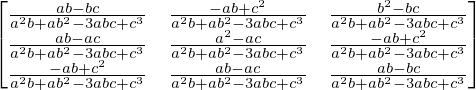
\includegraphics[width=1.4\textwidth]{inversa_m.png}
	\end{minipage}
\end{center}

Otra opción posible es crear un objeto simbolico matriz. La idea es crear una variable simbólica que contiene una matriz del tamaño que deseemos. Para ello empleamos el comando \mintinline{python}|MatrixSymbol|de \mintinline{python}|sympy.matrices|. Este comando admite un símbolo y dos parámetros numéricos que corresponden con el número de filas y columnas de la matriz creada. Estos parámetros tambień podrían a su vez ser simbólicos

\begin{center}
	\begin{minipage}{.3\textwidth}
		\begin{minted}{python}
In [56]: B = mt.MatrixSymbol('b',3,3)
B.shape
Out[60]: (3, 3)				
		\end{minted}
	\end{minipage}
\end{center}
Podemos obtener a partir de un objeto matriz simbólico la matriz simbólica de forma explícita,
\begin{center}
	\begin{minipage}{.3\textwidth}
\begin{minted}{python}
In [70]: B.as_explicit()
Out[70]:				
\end{minted}
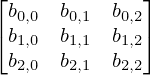
\includegraphics[width=0.8\textwidth]{matrixexp.png}		
	\end{minipage}
\end{center} 
podemos
Por último, el comando \texttt{sym} permite también convertir una expresión numérica en su equivalente simbólica,
\begin{verbatim}
>> a = [0.1 0.3 0.22
2.4 3 3.3
2 1 -1/3]
a =
    0.1000    0.3000    0.2200
    2.4000    3.0000    3.3000
    2.0000    1.0000   -0.3333

>> A = sym(a) 
A = 
[ 1/10, 3/10, 11/50]
[ 12/5,    3, 33/10]
[    2,    1,  -1/3]
\end{verbatim}



\subsection{Expresiones simbólicas}
Podemos ahora realizar operaciones aritméticas, con nuestras variables simbólicas,

\begin{center}
\begin{minipage}{.5\textwidth}
	\begin{minted}{python}
In [12]: q = 2*z + 2*x -y
In [13]: q
Out[13]: 			
	\end{minted}
	$4x - y$
\end{minipage}
\end{center}

\begin{paracol}{2}
El resultado es en este caso una expresión que guarda el resultado de la operación realizada. Es interesante notar cómo Sympy ha operado el contenido simbólico de las variables \texttt{x} y \texttt{z} para dar como resultado $4x$.

Para crear expresiones más complejas, Sympy tiene definidas las funciones matemáticas más comunes como funciones simbólicas,
\end{paracol}

\begin{center}
\begin{minipage}{.5\textwidth}
	\begin{minted}{python}
In [23]: expr = sp.cos(x)**2 + sp.sqrt(y) + sp.exp(x**2)
In [24]: expr
Out[24]: 			
	\end{minted}
	$\sqrt{y}+e^{x^2}+\cos^2(x)$
\end{minipage}
\end{center}

\begin{verbatim}
>> syms a b c x
>> y = a*x^2+b*x+c 
y = 
a*x^2 + b*x + c
 
>> rp = (-b+(b^2-4*a*c)^(1/2))/(2*a) 
rp = 
-(b - (b^2 - 4*a*c)^(1/2))/(2*a)
 
>> rm = (-b-(b^2-4*a*c)^(1/2))/(2*a) 
rm = 
-(b + (b^2 - 4*a*c)^(1/2))/(2*a)
\end{verbatim}

En este ejemplo, se han creado primero cuatro variables simbólicas y, a partir de ellas, se han generado tres expresiones simbólicas, la primera es un polinomio de grado dos y las dos siguientes las expresiones analíticas de sus raíces.

También es posible crear funciones simbólicas a partir de variables simbólicas, expresiones simbólicas o funciones matemáticas. Hay varias maneras de generarlas, pero quizá la más sencilla, es usar variables simbólicas previamente definidas,

\begin{verbatim}
>> syms x
f(x) = sin(x)
f(x) = 
sin(x)
\end{verbatim}

Las variables de la función se indican entre paréntesis a continuación del nombre de la función y antes del símbolo '\texttt{=}'. Si hay varias (posibles) variables y no se indica expresamente, Matlab tomará coma variable de la función aquella que alfabéticamente esté más cerca de la letra $x$. 

Es posible definir funciones de más de una variable,

\begin{verbatim}
>> syms x y
>> g(x,y)=sin(sqrt(x^2+y^2)) 
g(x, y) = 
sin((x^2 + y^2)^(1/2))
\end{verbatim}

o también, combinar funciones simbólicas mediante operadores aritméticos o composición de funciones, 
\begin{verbatim}
>> h(x,y) = f(x) - g(x,y)
h(x, y) =
sin(x) - sin((x^2 + y^2)^(1/2))
 
>> t(x) = g(x,y) ^f(x) 
t(x) = 
sin((x^2 + y^2)^(1/2))^sin(x)

>> r(x,y) = f(g(x,y)) 
r(x, y) = 
sin(sin((x^2 + y^2)^(1/2)))
\end{verbatim}

\subsection{Simplificación de expresiones simbólicas}
Matlab permite, dada una expresión simbólica, obtener una equivalente más sencilla. En general, este proceso de simplificación no es trivial ni unívoco, ya que una expresión puede admitir varias formas simplificadas. Es también posible que la expresión simbólica que deseamos simplificar, no sea simplificable.

Es interesante, sobretodo cuando se trata de expresiones obtenidas a partir de cálculos simbólicos, tratar de obtener una expresión lo más simplificada posible. La razón es que resulta mucho más fácil de entender y manipular. Matlab suministra el comando \texttt{simplify} para simplificar expresiones simbólicas. Así por ejemplo, si construimos la función simbólica,

\begin{verbatim}
>> f(x) = sin(x)^2 + cos(x)^2 
f(x) = 
cos(x)^2 + sin(x)^2
\end{verbatim} 

y le aplicamos el comando \texttt{simplify},
\begin{verbatim}
>> simplify(f)
ans(x) =
1
\end{verbatim}
Obtendremos un $1$, como cabría esperar. Este ejemplo es particularmente simple y, aunque sirve para ilustrar el funcionamiento del comando, no siempre es posible conseguir soluciones tan satisfactorias.

Veamos otro ejemplo que muestra la ambigüedad del comando \texttt{simplify},

\begin{verbatim}
>> syms x
>> p1 = 3*x^2+2*x-1
 
p1 =
 
3*x^2 + 2*x - 1
 
>> p1 = x^2-2*x+1
 
p1 =
 
x^2 - 2*x + 1
 
>> simplify(p1)
 
ans =
 
(x - 1)^2
\end{verbatim}

Matlab simplifica el polinomio de grado dos suministrado convirtiéndolo en un binomio. La pregunta que cabe hacerse es en qué medida podemos considerar el binomio una expresión simplificada del polinomio del que procede. Así por ejemplo, si estamos sumando polinomios, la expresión desarrollada resulta más \emph{simple} que la expresión binomial.

\subsection{Sustitución de variables por valores numéricos}
Es posible, una vez definida una expresión simbólica, sustituir sus variables por valores numéricos mediante el uso del comando \texttt{subs},

\begin{verbatim}
>> p = sin(x)^2 -2*x 
p = 
sin(x)^2 - 2*x
 
>> v = subs(p,2) 
v = 
sin(2)^2 - 4
\end{verbatim}

La variable \texttt{x} ha sido sustituida, en la expresión simbólica \texttt{p}, por el número $2$. La expresión resultante sigue siendo todavía simbólica.
Si lo que deseamos es obtener el valor numérico  de la función \texttt{p} en el punto $2$, tenemos que convertir la expresión simbólica resultante en su correspondiente valor numérico. Para ello se emplea el comando \texttt{double},

\begin{verbatim}
>> double(v)
ans =
   -3.1732
\end{verbatim}
Este comando toma su nombre del tipo de formato con que el ordenador va a representar el resultado; un número real guardado en doble precisión\footnote{En realidad Matlab convierte los resultados a números reales o complejos de acuerdo con la expresión simbólica de la que se han obtenido.}

Otro comando de interés para pasar de simbólico a numérico es el comando \texttt{vpa} (\emph{variable precision arithmetic}).
\begin{verbatim}
>> vpa(v) 
ans = 
-3.1731781895681940426804159084511
\end{verbatim}
El número de dígitos obtenidos al hacer la conversión es, por defecto, $32$. Dicho número puede ajustarse al 
valor que se desee introduciéndolo en \texttt{vpa} como un segundo parámetro,

\begin{verbatim}
>> vpa(v,5) 
ans = 
-3.1732
\end{verbatim}

Si una expresión engloba más  de una variable simbólica es posible sustituir solo alguna o algunas de ellas, para ello basta indicar el nombre de la variable que se desea sustituir seguida de su valor,
\begin{verbatim}
>> syms x y z

>> f = x^2*y + x * y^2 + z*x*y 
f = 
x^2*y + x*y^2 + z*x*y
 
>> fx = subs(f,x,2) 
fx = 
4*y + 2*y*z + 2*y^2
 
>> fy = subs(f,y,3) 
fy = 
9*x + 3*x*z + 3*x^2
 
>> fxz = subs(f,2,4) 
fxz = 
x^4*y + x*y^4 + z*x*y
\end{verbatim}
 
Además, es posible sustituir una variable simbólica por otra,

\begin{verbatim}
>> fxyx = subs(f,z,x) 
fxyx = 
2*x^2*y + x*y^2
 
>> f 
f = 
x^2*y + x*y^2 + z*x*y
 
>> fxxx = subs(fxyx,y,x) 
fxxx = 
3*x^3
\end{verbatim}


\section{Cálculo infinitesimal}
Es posible realizar operaciones típicas del cálculo infinitesimal como derivación e integración, empleando métodos de cálculo simbólico. A diferencia del cálculo numérico, el resultado será ahora una expresión. 

\subsection{Derivación}
Para obtener la derivada de una función simbólica, se emplea el comando \texttt{diff},
\begin{verbatim}
>> syms x a
>> f = a*exp(-x^2) 
f = 
a*exp(-x^2) 
>> df = diff(f) 
df = 
-2*a*x*exp(-x^2) 
\end{verbatim}
Matlab devuelve como resultado la derivada con respecto a la variable \texttt{x} de la función simbólica introducida. (Quizá sea útil recordar que Matlab toma como variable de la función la variable simbólica mas próxima alfabéticamente a la letra x.)

Si deseamos derivar una función respecto a una variable simbólica específica, es preciso indicarlo expresamente, introduciendo dicha variable en la llamada al comando \texttt{diff} a continuación de la función que vamos a derivar y separada de ésta por una coma. Así lo indicamos si queremos derivar la función del ejemplo anterior respecto a la variable simbólica \texttt{a},

\begin{verbatim}
>> dfa = diff(f,a) 
dfa = 
exp(-x^2)
\end{verbatim}

Es posible emplear el comando \texttt{diff} para obtener derivadas de orden superior. Para ello se introduce en la llamada el orden de la derivada a continuación del nombre de la función o, si es el caso, a continuación de la variable simbólica con respecto a la que se quiere derivar,

\begin{verbatim}
>> df3 = diff(f,3) 
df3 = 
12*a*x*exp(-x^2) - 8*a*x^3*exp(-x^2)
 
>> dfa2 = diff(f,a,2) 
dfa2 = 
0
\end{verbatim}

En el primer caso hemos obtenido la derivada tercera con respecto a \texttt{x} de la función \texttt{f} de los ejemplos anteriores y en el segundo la derivada segunda de dicha función con respecto a la variable \texttt{a}. 

Es fácil comprobar que el resultado sería el mismo si derivamos la función original y las expresiones de las sucesivas derivadas obtenidas hasta alcanzar la derivada del orden deseado,
\begin{verbatim}
>> df = diff(f) 
df = 
-2*a*x*exp(-x^2)
>> df2 = diff(df) 
df2 = 
4*a*x^2*exp(-x^2) - 2*a*exp(-x^2)
 
>> df3 = diff(df2) 
df3 = 
12*a*x*exp(-x^2) - 8*a*x^3*exp(-x^2) 
\end{verbatim}
En análisis matemático, cuando una función posee más de una variable independiente, la derivación respecto a una de sus variables recibe el nombre de derivada parcial. Así por ejemplo la función,
$f(x,y) =\sin \left( \sqrt{x^2+y^2} \right)$ es una función de dos variables $x$ e $y$. Su derivada (parcial) con respecto a $x$ y su derivada parcial con respecto a $y$, se representan como,
\begin{align*}
\frac{\partial f}{\partial x} &= x\cdot\frac{\cos(\sqrt{x^2+y^2})}{\sqrt{x^2+y^2}} \\
\frac{\partial f}{\partial y} &= y\cdot\frac{\cos(\sqrt{x^2+y^2})}{\sqrt{x^2+y^2}}
\end{align*}

Podemos obtener dichas derivadas parciales, indicando al comando \texttt{diff} respecto a qué variable debe derivar, tal y como se ha mostrado anteriormente, siendo en nuestro ejemplo con respecto a $x$ e $y$,
\begin{verbatim}
>> syms x y
>> fxy = sin(sqrt(x^2+y^2)) 
fxy = 
sin((x^2 + y^2)^(1/2))
 
>> sfx = diff(fxy,x) 
sfx = 
(x*cos((x^2 + y^2)^(1/2)))/(x^2 + y^2)^(1/2)
 
>> sfy = diff(fxy,y) 
sfy = 
(y*cos((x^2 + y^2)^(1/2)))/(x^2 + y^2)^(1/2)
\end{verbatim} 

Las derivadas parciales de orden superior pueden calcularse respecto a la misma o a distintas variables; por ejemplo para las derivadas segundas,

\begin{align*}
\frac{\partial^2f}{\partial x^2} &= \frac{\cos(\sqrt{x^2+y^2})}{\sqrt{x^2+y^2}} - 
x^2 \cdot \frac{\cos(\sqrt{x^2+y^2})}{\sqrt{(x^2+y^2)^3}} -
x^2 \cdot \frac{\sin(\sqrt{x^2+y^2})}{x^2+y^2} \\
\frac{\partial^2f}{\partial y^2} &= \frac{\cos(\sqrt{x^2+y^2})}{\sqrt{x^2+y^2}} - 
y^2 \cdot \frac{\cos(\sqrt{x^2+y^2})}{\sqrt{(x^2+y^2)^3}} -
y^2 \cdot \frac{\sin(\sqrt{x^2+y^2})}{x^2+y^2} \\
\frac{\partial^2f}{\partial x\partial y} &= \frac{\partial^2f}{\partial y\partial x} =-x\cdot y\cdot\frac{\cos(\sqrt{x^2+y^2})}{\sqrt{(x^2+y^2)^3}} - 
x\cdot y \cdot\frac{\sin(\sqrt{x^2+y^2})}{x^2+y^2} 
\end{align*}

Las derivadas calculadas respecto a variables distintas se llaman derivadas cruzadas, y no influye en ellas el orden en que se realice la derivación.

Para calcular las derivadas parciales de orden superior de una función, es suficiente indicar las variables con respecto a las cuales se desea derivar o, en el caso de que se calculen derivadas respecto a la misma variable, se puede también indicar el orden. En los siguientes ejemplos de código se muestra como obtener las derivadas segundas de la función que hemos venido utilizando a lo largo de esta sección empleando ambos métodos,
\begin{verbatim}
>> sfx2 = diff(fxy,x,x) 
sfx2 = 
cos((x^2 + y^2)^(1/2))/(x^2 + y^2)^(1/2)
-(x^2*cos((x^2 + y^2)^(1/2)))/(x^2 + y^2)^(3/2)
-(x^2*sin((x^2 + y^2)^(1/2)))/(x^2 + y^2)
 
>> sfx2 = diff(fxy,x,2) 
sfx2 = 
cos((x^2 + y^2)^(1/2))/(x^2 + y^2)^(1/2)
-(x^2*cos((x^2 + y^2)^(1/2)))/(x^2 + y^2)^(3/2)
-(x^2*sin((x^2 + y^2)^(1/2)))/(x^2 + y^2)
 
>> sfy2 = diff(fxy,y,y) 
sfy2 = 
cos((x^2 + y^2)^(1/2))/(x^2 + y^2)^(1/2)
-(y^2*cos((x^2 + y^2)^(1/2)))/(x^2 + y^2)^(3/2)
-(y^2*sin((x^2 + y^2)^(1/2)))/(x^2 + y^2)
 
>> sfy2 = diff(fxy,y,2) 
sfy2 = 
cos((x^2 + y^2)^(1/2))/(x^2 + y^2)^(1/2)
-(y^2*cos((x^2 + y^2)^(1/2)))/(x^2 + y^2)^(3/2) 
-(y^2*sin((x^2 + y^2)^(1/2)))/(x^2 + y^2)
 
>> sfxy = diff(fxy,x,y) 
sfxy = 
-(x*y*cos((x^2 + y^2)^(1/2)))/(x^2 + y^2)^(3/2)
-(x*y*sin((x^2 + y^2)^(1/2)))/(x^2 + y^2)
 
>> sfyx = diff(fxy,y,x) 
sfyx = 
-(x*y*cos((x^2 + y^2)^(1/2)))/(x^2 + y^2)^(3/2)
-(x*y*sin((x^2 + y^2)^(1/2)))/(x^2 + y^2) 
\end{verbatim}

Es posible emplear el comando de Matlab \texttt{pretty} para obtener una representación de una expresión simbólica más fácil de visualizar. Si la aplicamos al último de los resultados obtenidos en el ejemplo anterior obtenemos,

\begin{verbatim}
>> pretty(sfyx)
                2    2                   2    2
  x y cos(sqrt(x  + y ))   x y sin(sqrt(x  + y ))
- ---------------------- - ----------------------
         2    2 3/2                 2    2
       (x  + y )                   x  + y
\end{verbatim}

Es importante hacer notar que este comando no altera en modo alguno el valor de la expresión simbólica, simplemente la muestra por pantalla en un formato distinto.

Es posible emplear Matlab para realizar cálculos de gradientes, jacobianos, rotacionales, etc. No se incluye su descripción en este manual, los interesados pueden consultar la ayuda de Matlab.


\subsection{Integración} \index{Integración! Simbólica}
La integración indefinida en cálculo simbólico permite obtener la primitiva de una función dada,
\begin{equation*}
F(x) = \int f(x)dx  \Leftrightarrow f(x) = \frac{dF(x)}{dx}  
\end{equation*}
Se trata de una operación más compleja que la derivación. De hecho, hay funciones para las que no es posible obtener una primitiva en forma simbólica, bien porque no existe, o bien porque los algoritmos empleados por Matlab no son capaces de obtenerla.

El comando empleado para obtener la integral de una función es \texttt{int}. Así por ejemplo, para obtener la primitiva de la función $f(x) = \sqrt{1-x^2}$ haremos,
\begin{verbatim}
>> syms x
>> f = sqrt(1-x^2) 
f = 
(1 - x^2)^(1/2)
 
>> F = int(f)
F = 
asin(x)/2 + (x*(1 - x^2)^(1/2))/2
\end{verbatim}
Podemos comprobar el resultado obtenido aplicando la función \texttt{diff} vista en el apartado anterior,

\begin{verbatim}
>> diff(F) 
ans = 
1/(2*(1 - x^2)^(1/2)) - x^2/(2*(1 - x^2)^(1/2)) + (1 - x^2)^(1/2)/2
 
>> simplify(ans) 
ans = 
(1 - x^2)^(1/2)
\end{verbatim}
Donde se ha hecho uso del comando \texttt{simplify} para recuperar la expresión original.

Como en otras funciones simbólicas, \texttt{int} calcula la integral con respecto a la variable simbólica más próxima a \texttt{x}, salvo que se indique expresamente respecto a qué variable simbólica se desea integrar. Así por ejemplo,
\begin{verbatim}
>> syms x a

>> f = a * x/(a^2 +x^2) 
f = 
(a*x)/(a^2 + x^2)

>> Fx = int(f) 
Fx =
(a*log(a^2 + x^2))/2 

>> Fx = int(f,x) 
Fx = 
(a*log(a^2 + x^2))/2
 
>> Fa = int(f,a) 
Fa = 
(x*log(a^2 + x^2))/2 
\end{verbatim}
en el primer y el segundo caso la integración se realiza con respecto a la variable \texttt{x}. En el tercer caso, la integración se realiza respecto a la variable \texttt{a}.

Cuando no es posible encontrar una primitiva a una función, Matlab devuelve como resultado la expresión \texttt{int(integrando)}, para indicar que no ha sido posible realizar la operación,
\begin{verbatim}
>> f = sin(sinh(x)) 
f = 
sin(sinh(x))
 
>> F = int(f) 
F = 
int(sin(sinh(x)), x)
\end{verbatim}

La función \texttt{int}, puede emplearse también para calcular integrales definidas, si se le suministran los límites de integración,

\begin{verbatim}
>> f = 10 * sin(x) 
f = 
10*sin(x)
 
>> F0pi = int(f,0,pi) 
F0pi = 
20
\end{verbatim}

\subsection{Series} \index{Series! Simbólicas}
\index{Series! suma de series simbólicas}

\paragraph{Suma de series}Matlab permite calcular varias operaciones sobre sucesiones de las que se conoce el término general. En este capítulo, solo nos referiremos a la suma de series. 
Para ello se aplica el comando \texttt{symsum} indicando los límites de la serie que se quiere sumar,

\begin{verbatim}
>> syms k

>> symsum(1/k^2,1,inf)
pi^2/6

>> symsum((a)^k,0,inf)
ans =
piecewise([1 <= a, Inf], [abs(a) < 1, -1/(a - 1)])
\end{verbatim}
El segundo ejemplo muestra el límite de una serie geométrica, donde si $a>1$ la serie no converge. Como siempre, Matlab toma por defecto como variable (índice) la variable simbólica más próxima a \texttt{x}.

\paragraph{Serie de Taylor}\index{Series! Serie de Taylor de una función simbólica} Es posible calcular la expresión de la serie de Taylor para una función simbólica. Para ello se emplea el comando \texttt{taylor}. Por defecto se obtienen tan solo los elementos de la serie hasta orden 5, aunque es posible obtener órdenes superiores. A continuación se dan algunos ejemplos de uso,
\begin{verbatim}
>> syms x
>> f = exp(x)
 
f =
 
exp(x)
 
>> T = taylor(f)
 
T =
 
x^5/120 + x^4/24 + x^3/6 + x^2/2 + x + 1
 
>> T2 = taylor(f,x,1)
T2 =
exp(1) + exp(1)*(x - 1) + (exp(1)*(x - 1)^2)/2 + (exp(1)*(x - 1)^3)/6 +
(exp(1)*(x - 1)^4)/24 + (exp(1)*(x - 1)^5)/120
\end{verbatim}

Los ejemplos anteriores nos dan cinco términos del desarrollo de Taylor de la función exponencial. Primero en torno a $x = 0$, ya que no le hemos indicado un punto en torno al cual calcularlo. Después en torno a $x = 1$, valor definido en la llamada al comando \texttt{taylor} después del nombre de la función simbólica para la que queremos calcular el desarrollo.

Para calcular desarrollos de Taylor de otro orden distinto al quinto, debemos indicarlo expresamente, empleando en la llamada al comando \texttt{taylor} la palabra clave \texttt{'Order'}, seguida del orden que deseamos para la expansión,

\begin{verbatim}
>> T2 = taylor(f,x,'Order',7) 
T2 = 
x^6/720 + x^5/120 + x^4/24 + x^3/6 + x^2/2 + x + 1
\end{verbatim} 

\subsection{Límites} \index{Límites! de una función simbólica}
Para el cálculo de límites de una expresión simbólica se emplea el comando \texttt{limit}. Es necesario incluir la función simbólica y el valor de la variable independiente para el que se desea calcular el límite.  Dicho valor puede ser también simbólico,

\begin{verbatim}
>> syms x a

>> f =x^2/(3*x^2+log(x))
f =
 
x^2/(log(x) + 3*x^2)
>> limit(f,0)
ans = 
0
 
>> limit(f,a) 
ans = 
a^2/(log(a) + 3*a^2)

\end{verbatim}
Si la expresión para la que se desea calcular el límite tiene más de una variable simbólica, Matlab calculará el límite empleando como variable la más cercana a \texttt{x}, excepto si se le indica expresamente con respecto a qué variable debe calcularlo. El siguiente ejemplo muestra como emplear el comando \texttt{limit} y la definición de derivada para calcular la derivada de una función,

\begin{verbatim} 
>> syms h 
>> f = log(x)
 
f =
 
log(x)
 
>> limit (log(x+h)/h ,0)
 
ans =
 
log(h)/h
 
>> limit (log(x+h)/h ,h,0)
 
ans =
 
limit(log(h + x)/h, h == 0)
 
>> limit ((log(x+h)-log(x))/h ,h,0)
 
ans =
 
1/x
\end{verbatim}

Es posible calcular límites en el \emph{infinito}
\index{Límites! Límite en el infinito de una función simbólica}
\begin{verbatim}
>> limit (1/x,x,inf) 
ans = 
0
\end{verbatim}

Por último, es posible calcular el límite por la izquierda y el límite por la derecha cuando estos no coinciden. Para ello se añade al final del comando la palabra \texttt{'right} (derecha) o \texttt{'left'} (izquierda)
\index{Límites! Límites laterales de una función simbólica}
\begin{verbatim}
>> limit (1/x,x,0,'right') 
ans = 
Inf
 
>> limit (1/x,x,0,'left') 
ans = 
-Inf
 
>> limit (1/x,x,0) 
ans = 
NaN
\end{verbatim}
Es interesante notar que si no se especifica la dirección (left/right) al calcular este límite, el resultado es \texttt{NaN}; puesto que el límite, al no ser bilateral, no está bien definido.

\section{Representación gráfica}
Matlab dispone de un conjunto de funciones que permiten representar funciones simbólicas. Su funcionamiento es similar al de las funciones generales de Matlab para representación gráfica. A continuación se presenta una revisión de las más comunes.
\index{Gráficos! Representación de funciones simbólicas}
Para obtener la gráfica de una función de una sola variable se emplea el comando \texttt{ezplot}. Este comando admite como variables de entrada una función simbólica y un vector con los límites $[x_{min}\ x_{max}]$ entre los que se desea dibujar la función. Si no se suministran los límites, Matlab toma for defecto el intervalo $[-2\pi \ 2\pi]$ para realizar la representación. Así, por ejemplo para representar la función $f(x) = e^{\sin(x)}$,

%\begin{figure}
%\centering
%\subfigure[Intervalo por defecto: $-2\pi \leq x \leq 2\pi$ \label{fig:simplot1}]{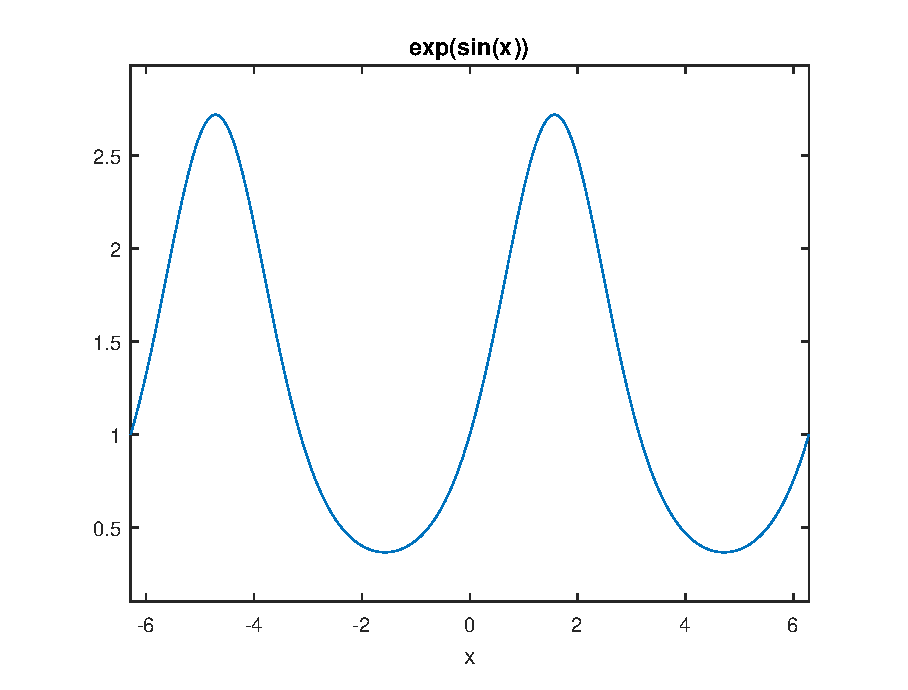
\includegraphics[width=9cm]{simplot.eps}} \qquad 
%\subfigure[Intervalo suministrado: $-10 \leq x \leq 10$  \label{fig:simplot2}]{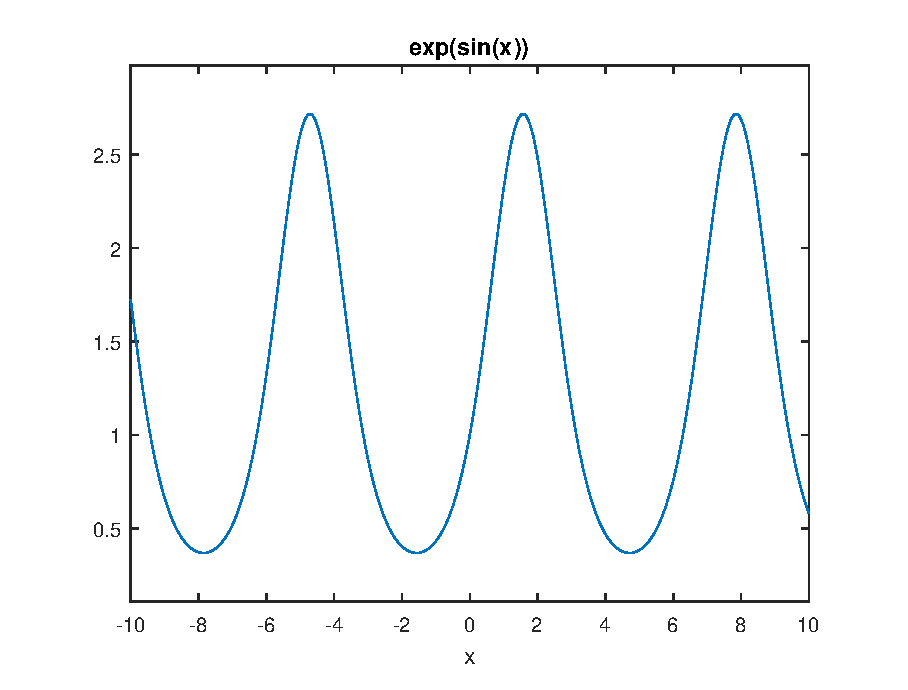
\includegraphics[width=9cm]{simplot2.eps}}\\
%\caption{Gráfica de la función $f(x) = e^{\sin\left(x\right)}$ obtenida a partir de su expresión simbólica con el comando \texttt{ezsurf} de Matlab}
%\end{figure}
\begin{figure}
	\centering
	\begin{subfigure}{0.45\textwidth}
		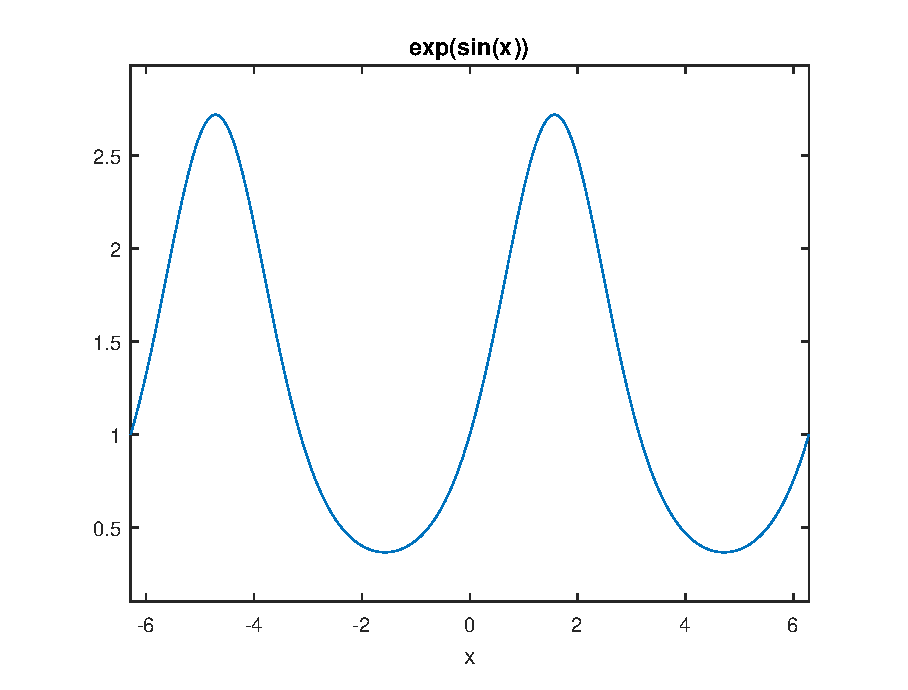
\includegraphics[width=10.5cm]{simplot.eps}
		\bicaption{Intervalo por defecto: $-2\pi \leq x \leq 2\pi$}{polynomials 2, 4, 6 and 8 degrees} \label{fig:simplot1}
	\end{subfigure} 
	\begin{subfigure}{0.45\textwidth}
		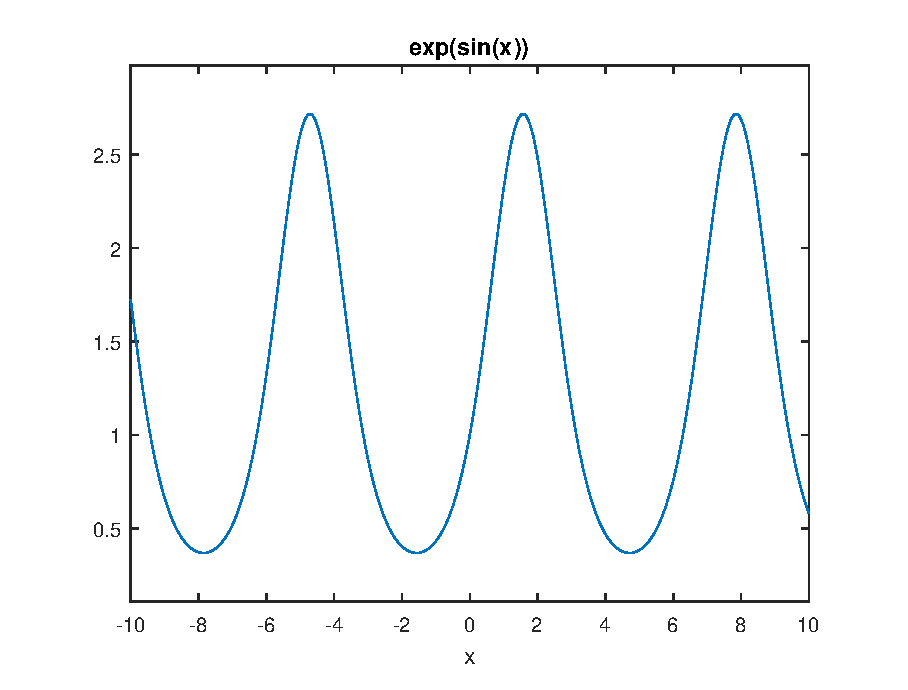
\includegraphics[width=10.5cm]{simplot2.eps}
		\bicaption{Intervalo suministrado: $-10 \leq x \leq 10$}{polynomials 2, 4, 6 and 8 degrees} \label{fig:simplot2}
	\end{subfigure}
	\bicaption{Gráfica de la función $f(x) = e^{\sin\left(x\right)}$ obtenida a partir de su expresión simbólica con el comando \texttt{ezsurf} de Matlab}{Taylor polynomial for cosine and sine functions}
\end{figure}
\begin{verbatim}
>> syms x

>> f = exp(sin(x)) 
f = 
exp(sin(x))
  
>> ezplot(f)

>> figure

>> ezplot(f,[-10 10])
\end{verbatim}
El resultado se muestra en la figuras \ref{fig:simplot1}, \ref{fig:simplot2}. 

La función \texttt{ezplot} puede emplearse también para representar curvas paramétricas, $x(t),\ y(t)$. Por ejemplo, $x(t) = t\cos(t),\  y(t)= t\sin(t)$ representa una espiral en el plano $x,\ y$. Para obtener su gráfica se debe pasar a \texttt{zplot} las funciones simbólicas $x(t)$ e $y(t)$,
\begin{verbatim}
>> syms t x y
>> x = t*cos(t)
x = 
t*cos(t)
 
>> y = t*sin(t) 
y = 
t*sin(t) 
>> ezplot(x,y)
\end{verbatim}

El resultado se muestra en la figura \ref{fig:simpar}. Si no se  indica un intervalo concreto para el parámetro \texttt{t}, Matlab toma por defecto el intervalo $[0 \ 2\pi]$. El intervalo puede especificarse mediante un vector $[t_{min} \ t_{max}]$ de modo análogo al caso de la representación de funciones de una sola variable. Una aplicación directa de la representación de curvas paramétricas es la obtención de la trayectoria de un móvil conocida su posición en función del tiempo. Por ejemplo, la obtención de la parábola trazada por un cuerpo que se mueve bajo la fuerza de la gravedad. 

\begin{figure}[h]
\centering
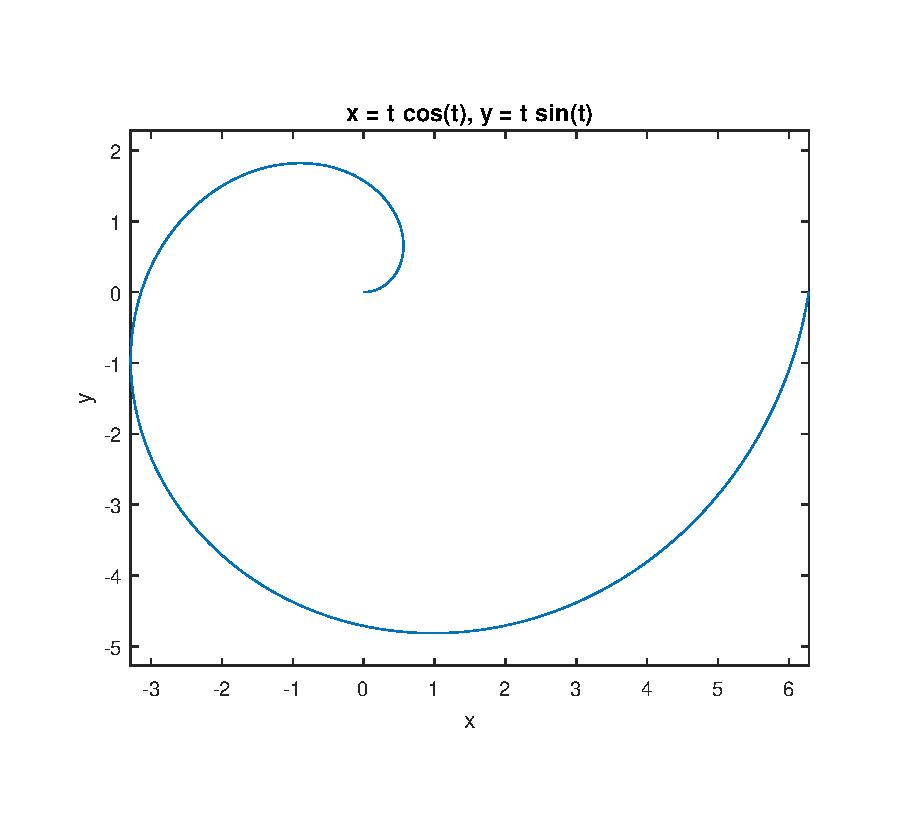
\includegraphics[scale=0.751]{simpar.eps}
\caption{Gráfica de la curva paramétrica $x(t) = t\cos(t), y(t)= t\sin(t)$ obtenida a partir de su expresión simbólica con el comando \texttt{ezsurf} de Matlab }
\label{fig:simpar}
\end{figure}

Por último es también posible representar superficies empleando funciones simbólicas de dos variables. Para ello se emplea el comando \texttt{ezsurf}. En este caso, es preciso suministrarle al menos la función de dos variables que se desea representar. Si no se especifica rango, Matlab por defecto representará la función en el intervalo $[-2\pi \ 2\pi]$, tanto para la abscisa como para la ordenada. Además, \texttt{ezsurf} admite como un segundo parámetro un vector de cuatro elementos $[x_{min} \ x_{max} \ y_{min} \ y_{max}]$ que indica el área sobre la que se quiere representar la función. Es posible también añadir un segundo parámetro al comando que especifica el tamaño de la retícula empleada para representar la superficie. Si no se indica este segundo parámetro, Matlab traza la superficie empleando una retícula de $60 \times 60$,


\begin{verbatim}
>> f = sin(sqrt(x^2+y^2))
f =
sin((t^2*vo^2 + (h0 - (a*t^2)/2)^2)^(1/2))
 
>> syms t x y
>> f = sin(sqrt(x^2+y^2))
f =
sin((x^2 + y^2)^(1/2))
 
>> ezsurf(f)
\end{verbatim}

La figura \ref{fig:surfsim} muestra los resultados de este ejemplo. 

\begin{figure}[h]
\centering
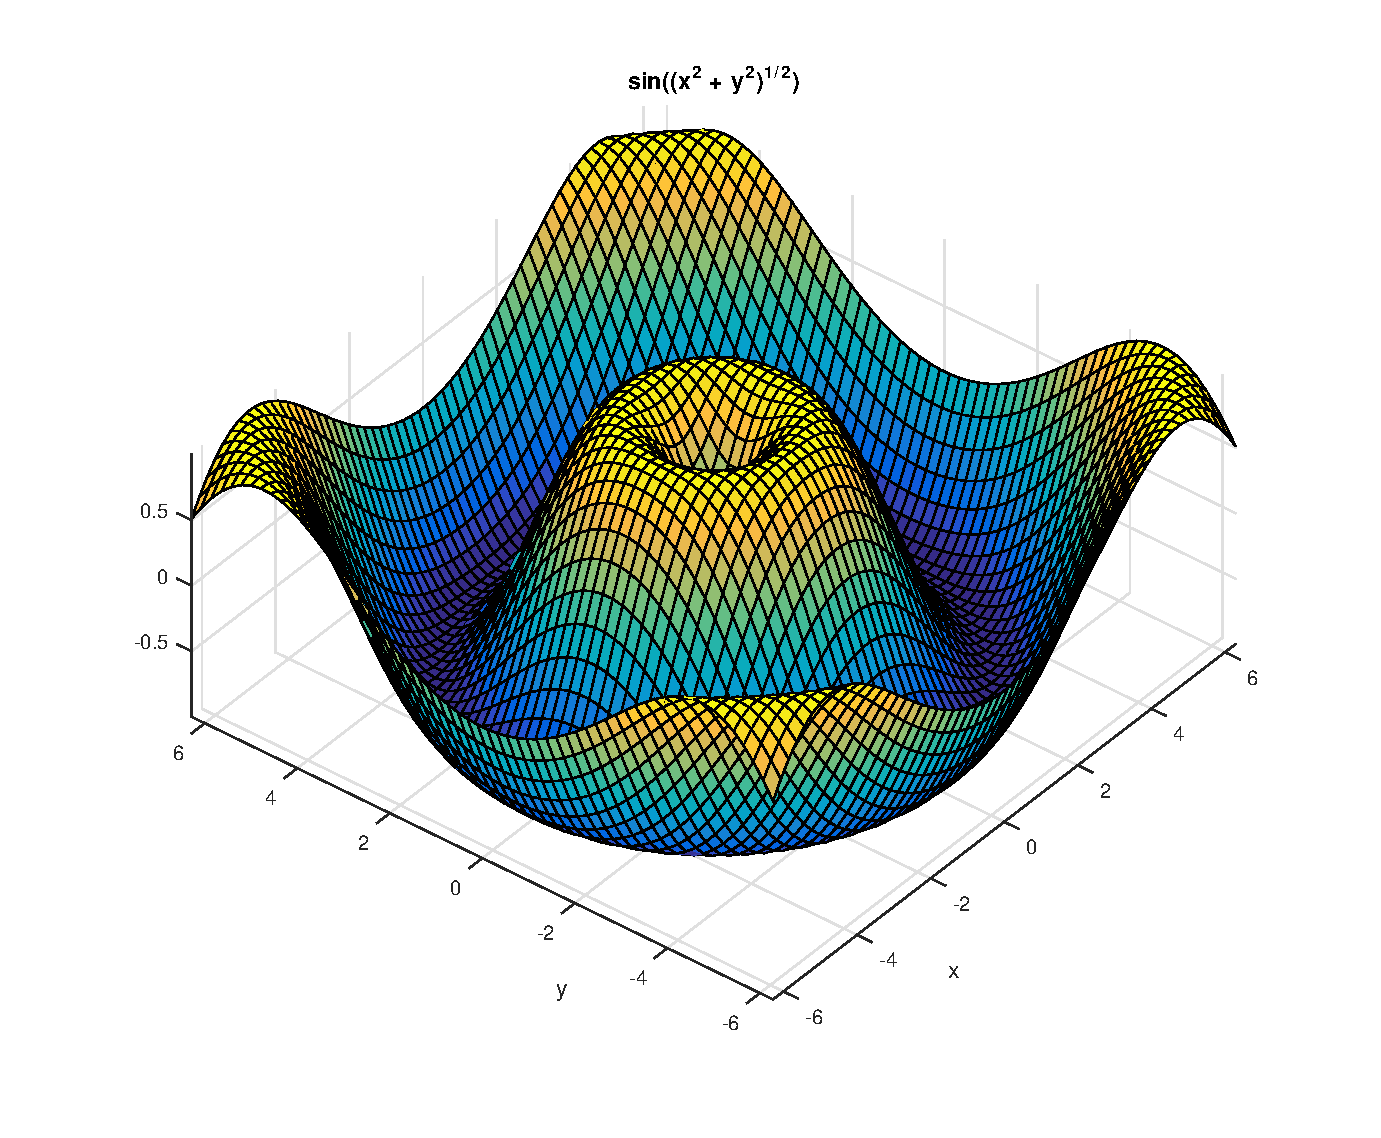
\includegraphics[scale=0.5]{surfsim.eps}
\caption{Gráfica de la función $f(x) = \sin\left(\sqrt{x^2+y^2}\right)$ obtenida a partir de su expresión simbólica con el comando \texttt{ezsurf} de Matlab }
\label{fig:surfsim}
\end{figure}

Hasta aquí la introducción al cálculo simbólico. Para obtener una visión completa de sus posibilidades se aconseja consultar la ayuda de Matlab






  

  	 